% http://en.wikibooks.org/wiki/LaTeX/Title_Creation
% Adjusted for EPFL template


\begin{titlepage}

\begin{center}

\raisebox{2cm}[-2cm][-2cm]{
\hspace{-1.5cm}

  \footnotesize
  \begin{tabular}{@{\hspace{0pt}}l@{\hspace{0pt}} l@{\hspace{10pt}}}
    \cline{1-1}     & \multirow{5}{*}{\hspace{10pt}\raisebox{-1ex}{
\includegraphics[width=0.4\columnwidth]{logo/logo}}}\\
    SWISS FEDERAL INSTITUTE OF TECHNOLOGY LAUSANNE  \\
    \cline{1-1} \\
    \raisebox{0.5ex}{\textbf{SCHOOL OF COMPUTER AND COMMUNICATION SCIENCES}} \\
    \raisebox{1.2ex}{COMPUTER SCIENCE SECTION| DISTRIBUTED INFORMATION SYSTEMS LABORATORY LSIR} \\
    %\scriptsize CH -- 1015 LAUSANNE \\

  \end{tabular}%
}

\vspace{1\baselineskip}
\Huge

\newcommand{\HRule}{\rule{\linewidth}{0.3mm}}


    {\huge \bfseries  A monolithic microrobotic arm \\ in silicon} \\
    {\Large \bfseries  Microrobot monolithique en silicium} \\
	\vspace{3mm}    
    \textsc{\Large Projet de Semestre} \Large (Automne 2009) \\
    \Large Section Microtechnique
    
    %\HRule \\[0.2cm]
	
	\vspace{3mm}
	%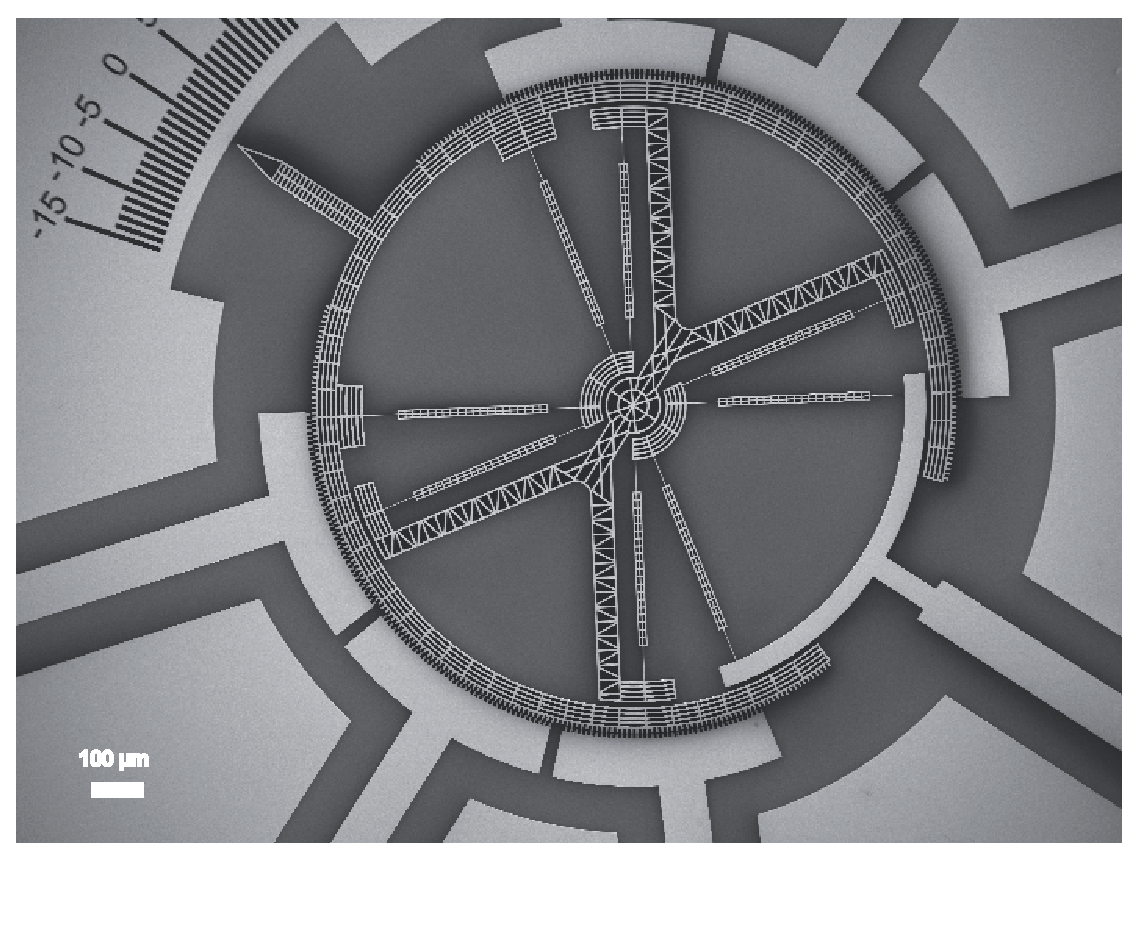
\includegraphics[height=6 cm]{fig_couverture}
	\vspace{3mm}
	\HRule 
	
	\emph{Author:} \\
	Arthur \textsc{Oviedo}\\
    \vspace{0.5cm}
    \emph{With the Supervision of:} \\   

    Prof. Karl \textsc{Aberer} \\   
    Eng. Nikolaos \textsc{Kasioumis}\\

	\vspace{0.5cm}
    % Bottom of the page
    \emph{21 January 2013}
	%{\large \today}


\end{center}


\end{titlepage}

\newpage
\thispagestyle{empty}
\mbox{}